% Appendix B

\chapter{Monitor Differences for \Qs} 
\captionsetup{justification=justified,singlelinecheck=false}

\label{AppendixB} 

\lhead{Appendix B. \emph{Monitor Differences}} 
This gives a summary of the monitor differences over Runs 1 and 2 (Wiens 1-9b) of \Q. The monitors shown are those used in the beam modulation analysis. The \Qs energy variable is also included since it is used in the Standard Regression scheme (see \ref{Chapter4}). Figures \ref{fig:Xdiff_by_slug} to \ref{fig:Ediff_by_slug} show the monitor differences averaged over slugs ($\sim$8~hr periods of the same IHWP slow-reversal state). Figures \ref{fig:Xdiff_by_wien} to \ref{fig:Ediff_by_wien} show the monitor differences averaged over Wiens ($\sim$1~month periods of the same Wien slow-reversal state). All averages are error-weighted with the same weights as the production dataset (MDallbars errors). The error bars shown come from the RMS width of the measured beam position and are thus mostly an indication of the beam properties as opposed to how accurately the differences in the beam parameters were measured. The precision of the measurements are given in Table \ref{tab:monitor_diff_by_wien} and are found by dividing the monitor resolution by the square root of the number of samples. A single BPM such as BPM3c12X has a resolution of approximately 1~$\mu$m. Studies were performed during \Qs to determine the resolution of the target variables which are composed of several BPM's extrapolated to the target position. The results of this study, found in the \Qs Analysis and Simulation Elog 788, are summarized in Table \ref{tab:res_mon}.
\begin{table}[h]
\begin{center}
\caption{\label{tab:res_mon}Resolution of target variables at the MPS ($\sim$1~ms) timescale. The larger resolutions in Run 2 are due to the failure of one of the BPM's used in the target variable composition. The resolution of helicity-correlated differences at quartet level are given by dividing these values by $\sqrt{2}$. The average values do not depend on the choice of errors (that is, errors derived from monitor resolution versus errors derived from RMS width of the differnce distribution) since the averaging weights come from the main detector error. Thus, these values correspond to the black dots in Figures \ref{fig:Xdiff_by_wien} to \ref{fig:Ediff_by_wien} even though the error bars are different.}
\begin{tabular}{lcc}\\\hline
~&Run 1&Run 2\\\hline\hline
targetX(Y)&0.98~$\mu$m&1.72~$\mu$m\\
targetXSlope(YSlope)&0.13~$\mu$rad&0.21~$\mu$rad\\
BPM3c12X(Y)&1.0~$\mu$m&1.0~$\mu$m\\\hline
\end{tabular}
\end{center}
\end{table}

\begin{landscape}
\begin{table}[h]
\begin{center}
\caption{\label{tab:monitor_diff_by_wien}Beam monitor helicity-correlated differences averaged over Wien states. The monitor differences are calculated at the runlet level and then weighted with the same weights as the production data to give the effective monitor differences. The errors are first calculated at the runlet level as the resolution of the monitors divided by the square root of the number of samples and then propagated using the same weights as the main detector production data. Resolutions used are the values in Table \ref{tab:res_mon} divided by $\sqrt{2}$ to account for quartet-level averaging.}
\begin{tabular}{|l|c|c|c|c|c|}\hline
Wien&targetX(nm)&targetXSlope(nrad)&targetY(nm)&targetYSlope(nrad)&bpm3c12X(nm)\\\hline\hline
1 &$4.32\pm 0.09$&$-0.15\pm 0.01$&$15.74\pm 0.09$&$0.71\pm 0.01$&$-3.71\pm 0.09$\\\hline
2 &$16.43\pm 0.07$&$-0.10\pm 0.01$&$-11.05\pm 0.07$&$0.48\pm 0.01$&$-40.95\pm 0.07$\\\hline
3 &$-19.56\pm 0.07$&$-0.66\pm 0.01$&$-5.21\pm 0.07$&$-0.34\pm 0.01$&$8.69\pm 0.08$\\\hline
4 &$-1.43\pm 0.08$&$-0.02\pm 0.01$&$-24.40\pm 0.08$&$-0.50\pm 0.01$&$6.77\pm 0.08$\\\hline
5 &$-15.42\pm 0.08$&$-0.62\pm 0.01$&$-7.23\pm 0.08$&$-0.63\pm 0.01$&$-10.97\pm 0.09$\\\hline
6 &$-2.96\pm 0.13$&$-0.11\pm 0.02$&$2.29\pm 0.13$&$0.05\pm 0.02$&$14.25\pm 0.08$\\\hline
7 &$10.58\pm 0.16$&$0.26\pm 0.02$&$7.31\pm 0.16$&$0.17\pm 0.02$&$-18.95\pm 0.09$\\\hline
8a&$-16.51\pm 0.11$&$-0.42\pm 0.01$&$-6.77\pm 0.11$&$-0.37\pm 0.01$&$-0.23\pm 0.07$\\\hline
8b&$2.19\pm 0.11$&$0.05\pm 0.01$&$0.60\pm 0.11$&$-0.04\pm 0.01$&$4.41\pm 0.06$\\\hline
9a&$0.23\pm 0.09$&$0.02\pm 0.01$&$3.22\pm 0.09$&$0.05\pm 0.01$&$-0.02\pm 0.05$\\\hline
9b&$-0.88\pm 0.09$&$-0.02\pm 0.01$&$-2.59\pm 0.09$&$-0.10\pm 0.01$&$-1.09\pm 0.05$\\\hline
\end{tabular}
\end{center}
\end{table}
\end{landscape}
\begin{figure}
\centering
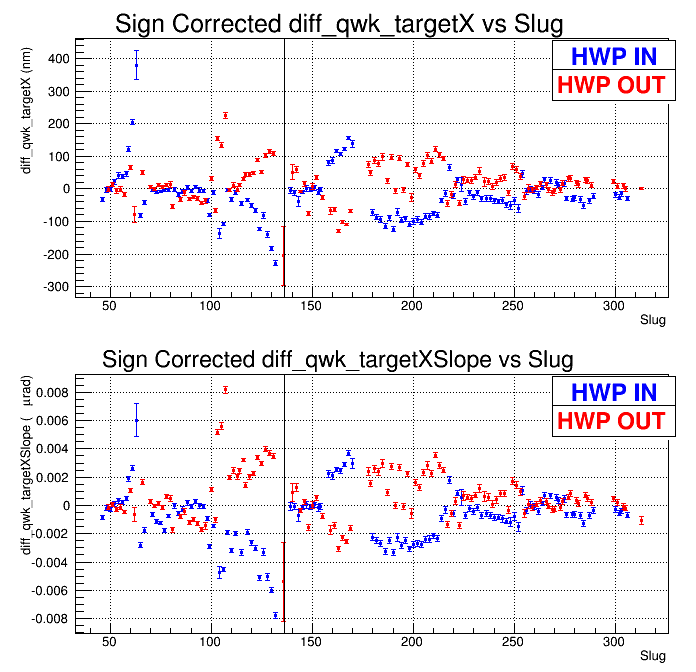
\includegraphics[width=5.9in]{./Pictures/XDifferences_by_Slug.png}
\caption{\label{fig:Xdiff_by_slug}Slug-averaged helicity-correlated differences in horizontal position (top) and angle (bottom) at the target color-labeled by half-wave plate state. The errors shown are derived from monitor difference RMS widths and reflect beam motion not measurement precision.}
\end{figure}

\begin{figure}
\centering
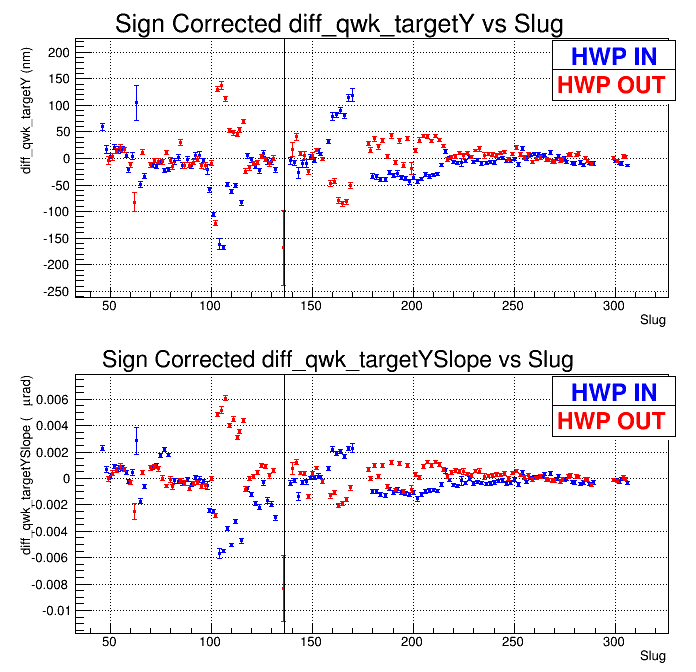
\includegraphics[width=5.9in]{./Pictures/YDifferences_by_Slug.png}
\caption{\label{fig:Ydiff_by_slug}Slug-averaged helicity-correlated differences in vertical position (top) and angle (bottom) at the target color-labeled by half-wave plate state. The errors shown are derived from monitor difference RMS widths and reflect beam motion not measurement precision. }
\end{figure}

\begin{figure}
\centering
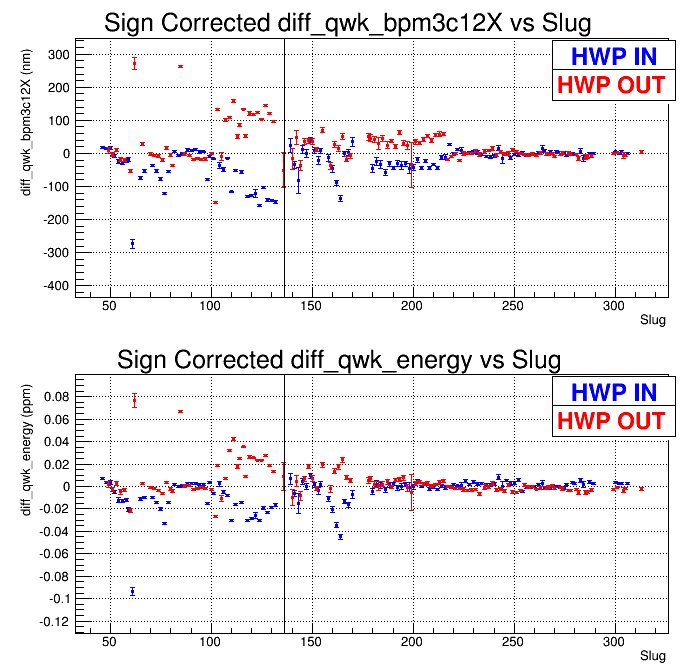
\includegraphics[width=5.9in]{./Pictures/EDifferences_by_Slug.png}
\caption{\label{fig:Ediff_by_slug}Slug-averaged helicity-correlated differences in horizontal position at BPM3c12X (top) and \Qs energy variable (bottom) color-labeled by half-wave plate state. The errors shown are derived from monitor difference RMS widths and reflect beam motion not measurement precision.}
\end{figure}

\begin{figure}
\centering
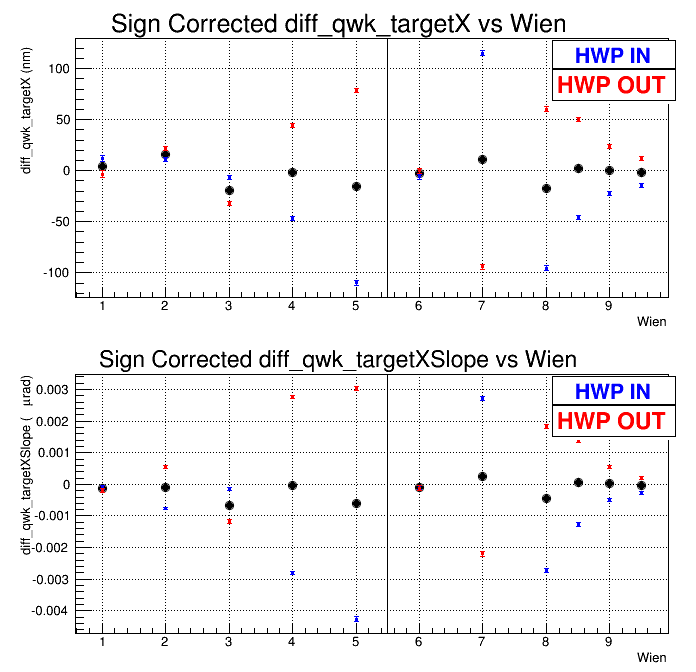
\includegraphics[width=5.9in]{./Pictures/XDifferences_by_wien.png}
\caption{\label{fig:Xdiff_by_wien}Wien-averaged helicity-correlated differences in horizontal position (top) and angle (bottom) at the target color-labeled by half-wave plate state. The average of the In and Out IWHP states is shown in black. The errors shown are derived from monitor difference RMS widths and reflect beam motion not measurement precision. For measurement precision estimates see Table \ref{tab:monitor_diff_by_wien}.}
\end{figure}

\begin{figure}
\centering
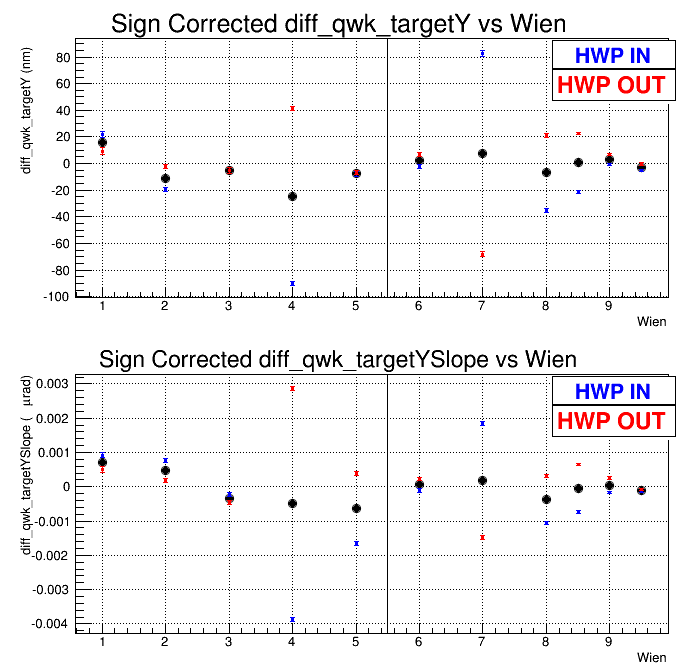
\includegraphics[width=5.9in]{./Pictures/YDifferences_by_wien.png}
\caption{\label{fig:Ydiff_by_wien}Wien-averaged helicity-correlated differences in vertical position (top) and angle (bottom) at the target color-labeled by half-wave plate state. The average of the In and Out IWHP states is shown in black. The errors shown are derived from monitor difference RMS widths and reflect beam motion not measurement precision. For measurement precision estimates see Table \ref{tab:monitor_diff_by_wien}. }
\end{figure}

\begin{figure}
\centering
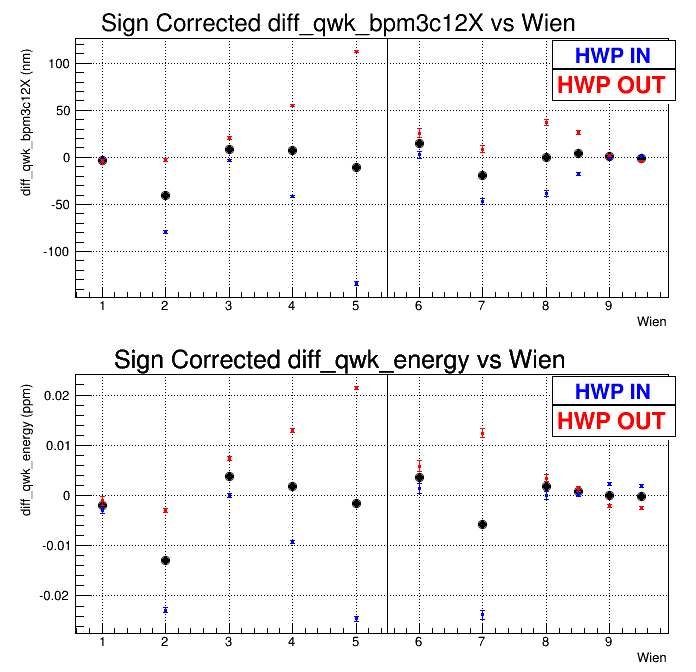
\includegraphics[width=5.9in]{./Pictures/EDifferences_by_wien.png}
\caption{\label{fig:Ediff_by_wien}Wien-averaged helicity-correlated differences in horizontal position at BPM3c12X (top) and \Qs energy variable (bottom) color-labeled by half-wave plate state. The average of the In and Out IWHP states is shown in black. The errors shown are derived from monitor difference RMS widths and reflect beam motion not measurement precision. For measurement precision estimates see Table \ref{tab:monitor_diff_by_wien}.}
\end{figure}
